\section{ROS} \label{sec:ros}
Aquí se explicará un poco sobre qué es ROS.
\begin{figure}[h]
	\centering
	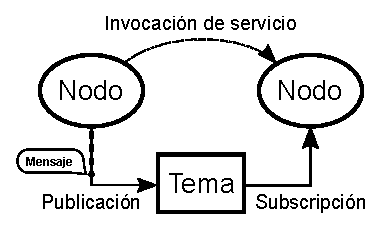
\includegraphics[width=0.5\linewidth]{img/ROS_concepts}
	\caption{Diagrama de comunicación de ROS}
	\label{fig:rosconcepts}
\end{figure}

También están interesantes las animaciones que vienen en la \href{https://docs.ros.org/en/humble/Tutorials/Beginner-CLI-Tools/Understanding-ROS2-Topics/Understanding-ROS2-Topics.html}{página de ROS} \cite{ros2-understanding-topics}, pero lamentablemente no se pueden poner animaciones en el reporte.

\subsection{Nodo (Node)}
\subsection{Tema (Topic)}
\subsection{Mensaje (Message)}
\subsection{Servicio (Service)}
\subsection{Gazebo}
\subsection{RViz}
